\section{Data}\label{data}
\begin{table*}
    \caption{Examples of \todo{matching} argument key point pairs from the \ArgKP dataset~\cite{Bar-HaimEFKLS2020}}
    \label{examples}
    \begin{tabularx}{\linewidth}{lXp{4.3cm}c}
      \toprule
      \textbf{\#} & \textbf{Argument} & \textbf{Key point} \\
      \midrule
      A & % from training set, match
      child \textcolor{violet}{actors} can be overworked and they can miss out on their education. & % arg_13_153
      Being a \textcolor{violet}{performer} harms the child's education \\ % kp_13_5
      B & % from training set, match
      as long as nuclear weapons exist, the entire world has to worry about \textcolor{violet}{nations} deciding to fire them at another or \textcolor{violet}{terrorists} getting hold of them and causing disaster & % arg_17_91	
      Nuclear weapons can fall into the \textcolor{violet}{wrong hands} \\ % kp_17_1
      C & % from training set, not labelled
      `people reach their limit when it comes to their quality of life and should be able to end their \textcolor{violet}{suffering}. this can be done with little or no \textcolor{violet}{suffering} by \textcolor{teal}{assistance} and the person is able to say good bye. & % arg_0_0
      \textcolor{teal}{Assisted} suicide reduces \textcolor{violet}{suffering} \\ % kp_0_1
      \bottomrule
    \end{tabularx}
  \end{table*}

\begin{figure*}
    \centering
    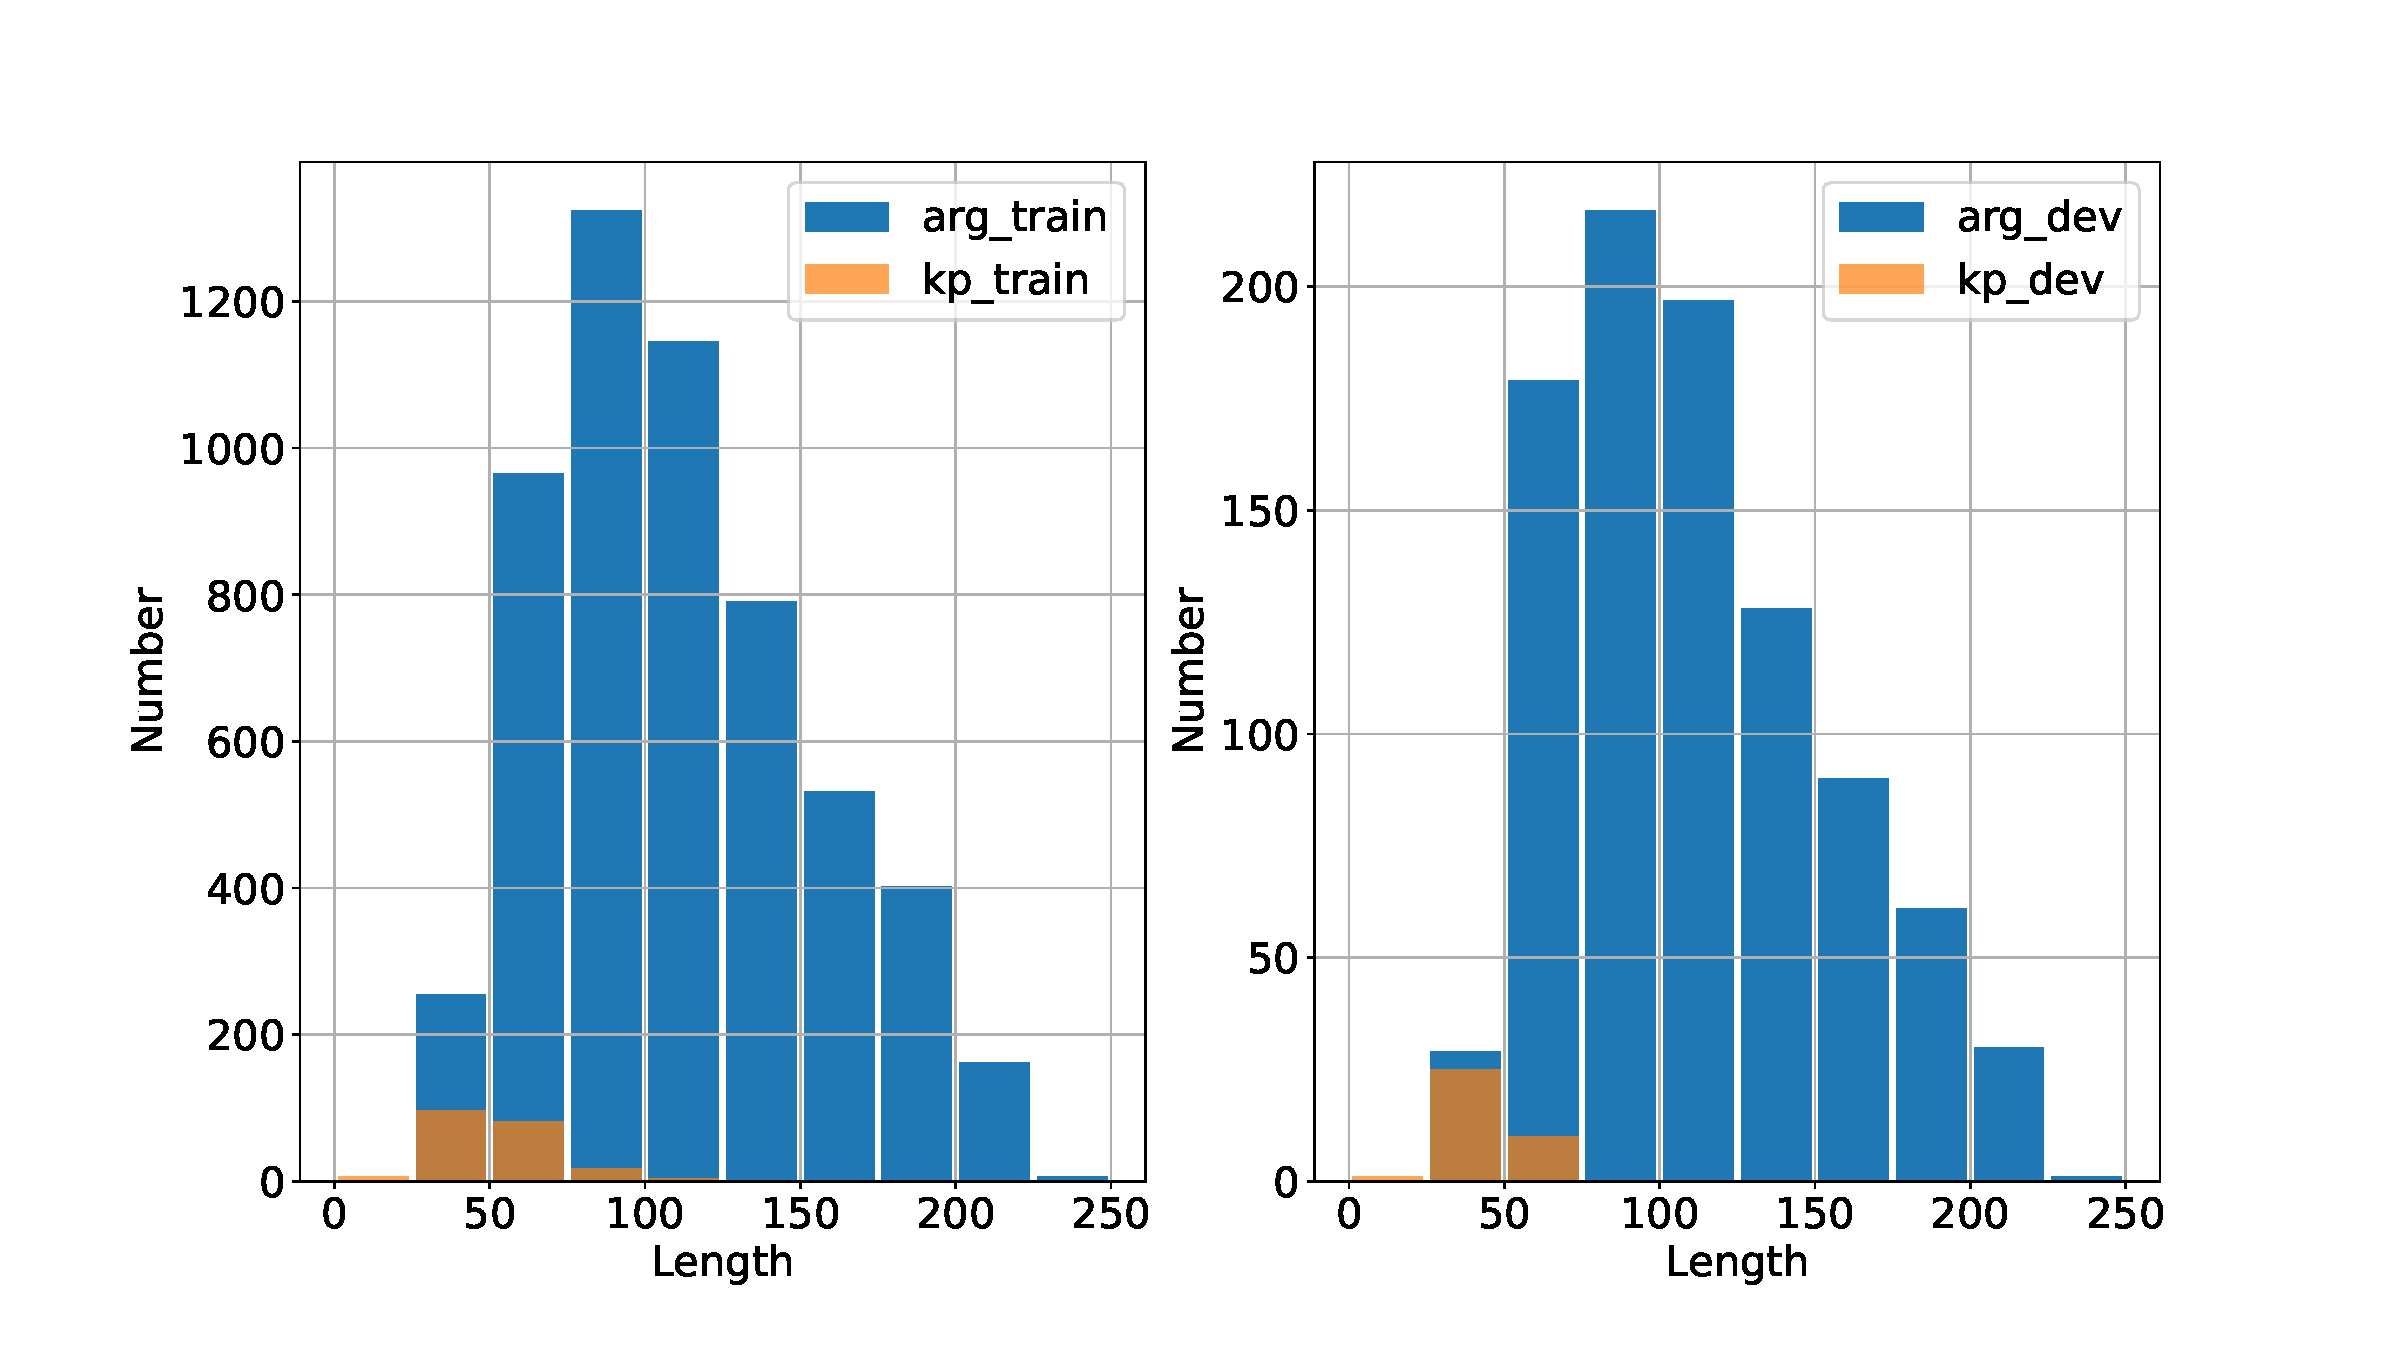
\includegraphics[width=\linewidth]{arg-kp-length.pdf}
    \caption{Lengths in characters for arguments and key points from the training and development set.}
    \label{arg-kp-length}
\end{figure*}

The dataset used in the ArgMining 2021 shared task on Quantitative Summarization and Key Point Analysis is the \ArgKP dataset~\cite{Bar-HaimEFKLS2020} which consists of 24\,083 argument 
and key point pairs labeled as matching/non-matching. They all belong to one of 28~controversial topics, for example: 
\textquote{Assisted suicide should be a criminal offence}. Every key point and argument pair is annotated with its stance towards the topic. 

The training split of the \ArgKP dataset has 5\,583~arguments belonging to 207~key points within 24~topics. This leaves the validation split with 932~arguments and 36~key points for 4~topics.
\citet{kpa-2021-overview} complement the \ArgKP dataset's training and validation split with a test split that is used to evaluate submissions to the shared task. The test split contains 723~arguments with 33~key points from 3~topics.

\subsection{Characteristics}

We analyze the \ArgKP dataset and observe that matched and unmatched key points of a given argument both contain very frequent words. 
Many of these are stopwords such as \textquote{as}, \textquote{for}, and \textquote{not} and are very common in natural language.
Because of their high frequency, stop words tend to be less distinctive in assessing the semantic similarity of two texts, especially while using bag-of-words to represent texts.
We therefore remove stop words from our data during preprocessing arguments and key points for our baseline. 
Furthermore, important words found in arguments are repeated with different tenses and parts of speech in key points, for example: 
\textquote{legalize}, \textquote{legalized}, \textquote{legalizing}, and \textquote{legal}. 
To resolve ambiguities in the vocabulary, such words are normalized with a stemming method in our approach.

In Table~\ref{examples} we show examples of argument key point pairs from the \ArgKP dataset~\cite{Bar-HaimEFKLS2020}. 
We identify the following major difficulties in matching key points to arguments: semantically similar words and meaning 
understanding.
In pair~A from Table~\ref{examples}, the argument matches the given key point. Both sentences discuss 
children actors and their education. The word \textquote{actors} is not explicitly used in the key point but is 
semantically similar to the word \textquote{performer}. 
In our baseline, we oppose this challenge by using the well-known lexical database WordNet~\cite{Miller1995} in our 
baseline to find synonyms and antonyms.
In pair~B from Table~\ref{examples}, the argument matches the key point but are expressed differently. 
The key point makes usage of \textquote{wrong hands} as figurative meaning for \textquote{nations} and \textquote{terrorists} from the argument. 
To predict if a key point is aligned with some argument, we need to understand their meanings and compare them. 
To better deal with this problem, we use two well-known language models in our second approach~(Section~\ref{approach}). 

We further observe in Figure~\ref{arg-kp-length} that arguments from the \ArgKP dataset are longer than key points.
In the training set, the average length of arguments is 109~characters. 
Compared to that, key points are on average only half as long (52~characters). 
In the validation set, the key points have an average length of 41~characters and therefore key points are shorter than those in the training set. 
The average length of arguments remains almost the same at 108~characters. 
%The differences in length between arguments and key points from the training set and validation set are~57.8 characters and~66.3 characters respectively. 
The proportion of arguments that are 67~characters longer than key points constitute 39\,\%~of the training set 
and 44\,\% of the validation set. 
We can see that there are more short key points in the validation set. 
This length difference might be a challenge for the models in key point matching~(Section~\ref{error-analysis}).
